\documentclass[diplomskirad]{fer}

\usepackage{booktabs}
\usepackage{listings}
\usepackage[outputdir=out]{minted}

\newcommand{\paragraphnewline}[1]{\paragraph{#1}\mbox{}\\}


\title{Dynamic fluid visualization using smoothed particle hydrodynamics method}
\naslov{Vizualizacija dinamike fluida metodom hidrodinamike zaglađujućih čestica}
\brojrada{542}
\mentor{Krešimir Trontl}
\author{Hrvoje Hemen}
\date{June, 2024}
\datum{lipanj, 2024.}
\begin{document}
    \maketitle
    \zadatak{HrvojeHemenZadatak.pdf}
    \begin{zahvale}
        Želim se zahvaliti mentoru Krešimiru Trontlu-
    \end{zahvale}
    \mainmatter
    \tableofcontents
% TEKST RADA


    \chapter{Uvod}\label{ch:uvod}


    \section{Cilj rada}\label{sec:cilj-rada}

    Cilj ovog rada bio je napraviti realnu simulaciju dinamike fluida.
    Korištena metoda bila je metoda hidrodinamike zaglađujućih čestica (SPH).
    Inspiracija za ovaj rad bio je jedan YouTube video Sebastiana Laguea koji govori o simulaciji vode u Unityju.


    \section{Ukratko o radu}\label{sec:ukratko-o-radu}

    U sklopu ovog rada obrađeno je sve potrebno za samostalnu izradu ovog rada uključujući i postavljanje razvojnog okruženja.

    Rad je pisan u c\# programskom jeziku u sklopu Unityja, te je za vizualizaciju korišten Unityjev dvodimenzionalni vizualizator.


    \chapter{Tehnologije}\label{ch:tehnologije}


    \section{C\#}\label{sec:c}

    \begin{figure}[H]
        \centering
        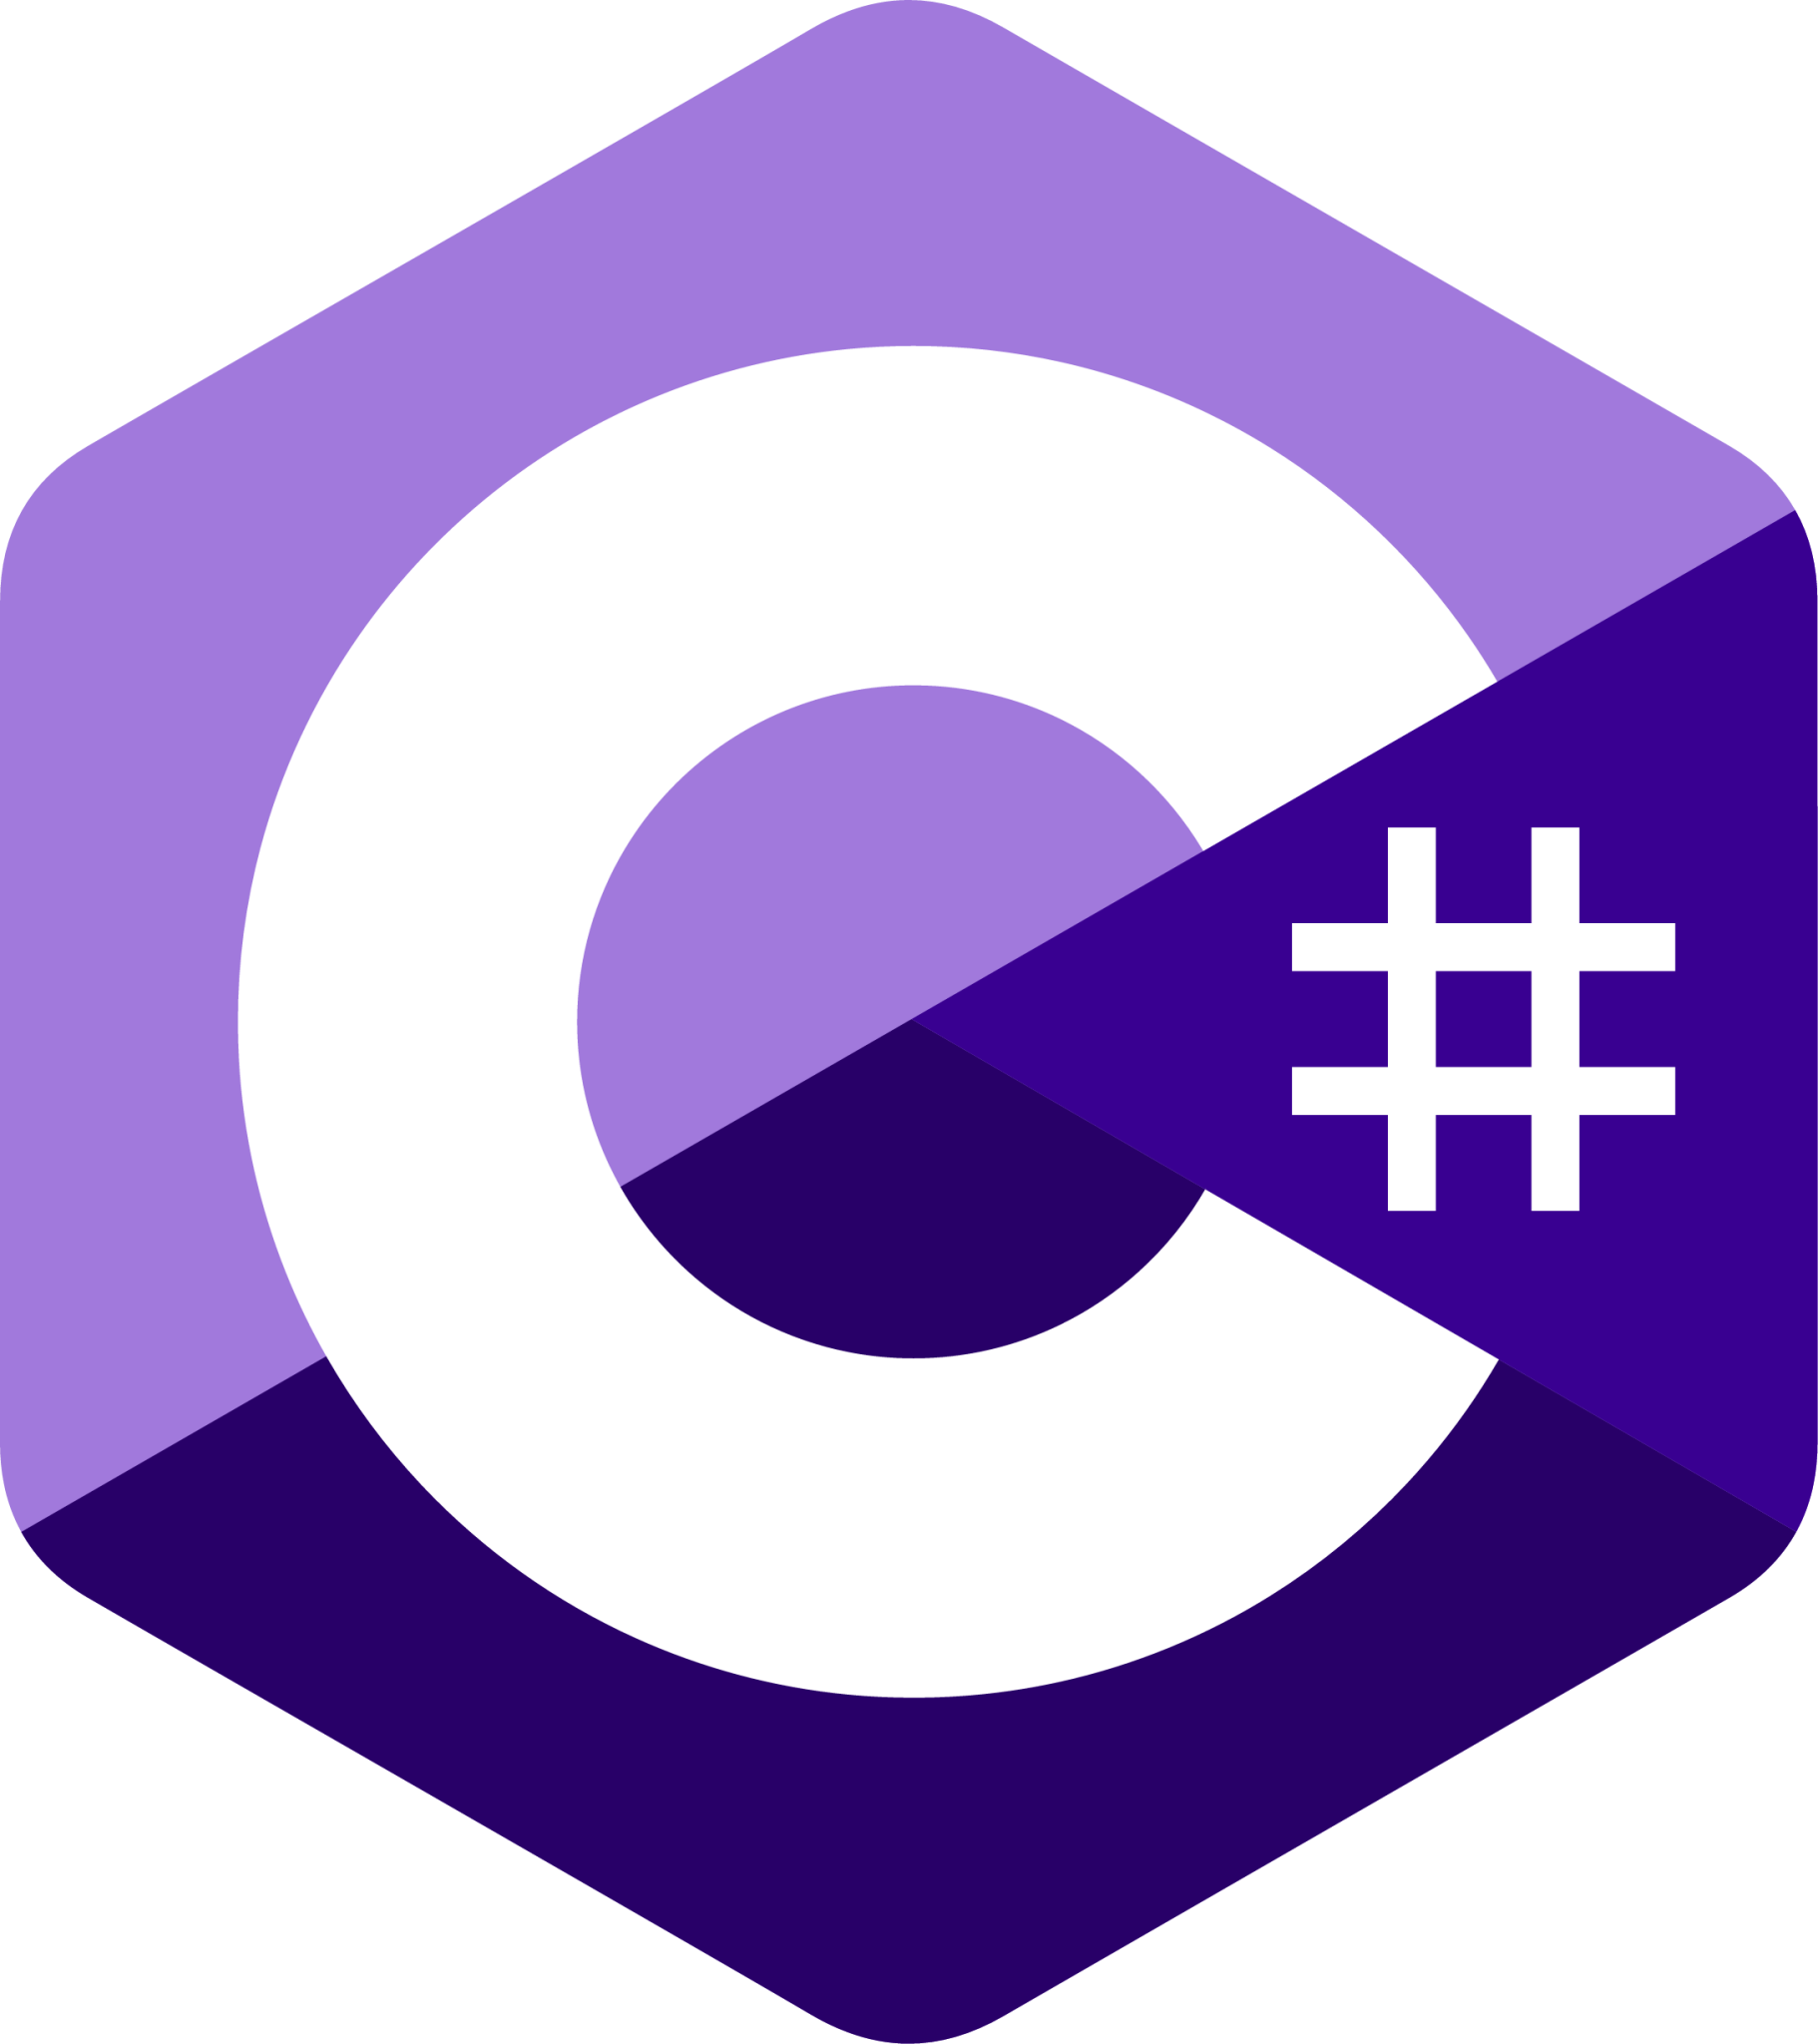
\includegraphics[scale=0.1]{images/c-sharp}
        \caption{
            C Sharp Logo \cite{cSharpLogo}
        }
        \label{fig:cSharpLogo}
    \end{figure}

    C\# ("C-sharp") je objektno orijentirani programski jezik visoke razine razvijen od strane Microsofta.
    Jezik je nastao ranih 2000-ih kao dio .NET inicijative, s ciljem da kombinira računalnu snagu C++ s jednostavnošću i sigurnošću Jave.

    \begin{itemize}
        \item \textbf{Razvoj i povijest:} C\# je prvi put predstavljen 2000\. godine i brzo je postao popularan zbog svoje sličnosti s C i C++ jezicima,
        kao i zbog svoje integracije s .NET frameworkom.
        Jezik je dizajniran kako bi bio jednostavan za učenje, strogo tipiziran i prijenosan na različite operacijske sustave.
        \item \textbf{Sintaksa i struktura:} C\# sintaksa je vrlo slična onoj u Javi, gdje svaka naredba završava sa točka-zarezom (\texttt{;}).
        Kod je organiziran u klase i metode, a dijelovi koda su omeđeni vitičastim zagradama (\{\}).
        Jedna od ključnih razlika između C\# i Jave je mogućnost preopterećenja osnovnih operacija u C\#.
        Na primjer, možete definirati kako se operator \texttt{+} ponaša za prilagođene klase.
        \item \textbf{Prednosti i upotreba:} C\# je vrlo moćan jezik s mnogim značajkama kao što su LINQ (Language Integrated Query),
        async/await za jednostavno upravljanje asinkronim operacijama, i podrška za razne paradigme programiranja uključujući objektno orijentirano,
        funkcionalno i imperativno programiranje.
        \item \textbf{Integracija s Visual Studio:} C\# je potpuno integriran s Visual Studio, jednim od najmoćnijih razvojnih okruženja, što omogućava brzi razvoj, testiranje i implementaciju aplikacija.
        \item \textbf{Ekosustav i knjižice:} C\# ima bogat ekosustav knjižica kao što su ASP.NET za web razvoj, Xamarin za mobilne aplikacije, te Unity za razvoj igara.
    \end{itemize}


    \newpage


    \section{Unity}\label{sec:unity}

    \begin{figure}[H]
        \centering
        
\includegraphics[scale=0.3]{images/unityLogo}
        \caption{
            Unity Logo \cite{unityLogo}
        }
        \label{fig:unityLogo}
    \end{figure}

    Unity je razvojno okruženje i pogonski sklop za igre koje omogućava razvoj 2D, 2.5D i 3D igara.
    Od svog nastanka 2005\. godine, Unity se kontinuirano razvija i postaje jedan od najpopularnijih alata za razvoj igara na tržištu.

    \begin{itemize}
        \item \textbf{Razvoj i povijest:} Unity je lansiran 2005.
        godine s ciljem da olakša razvoj igara, pružajući pristupačne alate i dokumentaciju za programere svih razina vještina.
        Od tada, Unity je narastao i zauzeo značajan udio na tržištu razvoja igara.
        \item \textbf{Platforme i podrška:} Jedna od najvećih prednosti Unityja je njegova sposobnost razvoja za različite platforme, uključujući mobilne uređaje, desktop, web, konzole i virtualnu stvarnost.
        To omogućava programerima da razvijaju igre koje mogu biti lako prenesene i distribuirane na više platformi.
        \item \textbf{Licenciranje i pristupačnost:} Unity nudi nekoliko razina licenci, uključujući besplatnu verziju koja omogućava novim programerima ulazak u svijet razvoja igara.
        Besplatna verzija je opsežna i omogućava programerima da istraže sve značajke Unityja bez početnih troškova.
        \item \textbf{Dokumentacija i zajednica:} Unity je poznat po svojoj opsežnoj dokumentaciji i aktivnoj zajednici.
        Mnogi resursi, kao što su forumi, vodiči, tečajevi i online podrška, dostupni su kako bi pomogli programerima da brzo nauče i rješavaju probleme.
        \item \textbf{Alati i integracija:} Unity nudi širok spektar alata za razvoj, uključujući svoj IDE, alate za animaciju, nativni fizički simulator, te podršku za nadogradnje razvojene od strane drugih ljudi.
        \item \textbf{Renderiranje i grafika:} Unity koristi napredne tehnike renderiranja i grafičke mogućnosti, uključujući podršku za High Definition Render Pipeline (HDRP) i Universal Render Pipeline (URP), što omogućava visoku kvalitetu vizualnih efekata i performansi na raznim uređajima.
    \end{itemize}


    \chapter{Teorijska podloga}\label{ch:teorijska-podloga}


    \section{Pristupi računalnoj simulaciji fluida}\label{sec:pristupi-racunalnoj-simulaciji-fluida}

    Kada govorimo o simulaciji fluida, postoji nekoliko različitih pristupa koji se koriste u računalnim znanostima i inženjerstvu.
    Ovaj rad se fokusira na SPH (Smoothed Particle Hydrodynamics) metodu, no važno je razumjeti širi spektar tehnika koje su dostupne i njihove primjene.
    U ovom poglavlju, raspravit ćemo o najvažnijim metodama simulacije fluida, njihovim karakteristikama, prednostima i nedostacima.

    \subsection{Simulacije bazirane na česticama}\label{subsec:simulacije-bazirane-na-cesticama}

    Simulacije bazirane na česticama su jedne od najintuitivnijih i najčešće korištenih metoda za simulaciju fluida.
    U ovim metodama, svaka čestica predstavlja mali dio fluida, kao što je kapljica vode, te nosi svojstva kao što su masa, brzina i vektor smjera kretanja.
    Ove simulacije omogućavaju vrlo detaljan i dinamičan prikaz tekućina.

    \begin{itemize}
        \item \textbf{Osnovni princip:} Svaka čestica ima svoje fizičke karakteristike koje se koriste za izračunavanje među-čestičnih sila poput tlaka, gustoće i viskoznosti. Na temelju tih sila, simulacija izračunava nova svojstva čestica za svaki korak simulacije. Ovaj proces se ponavlja iterativno, omogućujući simulaciji da prikaže dinamiku fluida kroz vrijeme.
        \item \textbf{SPH (Smoothed Particle Hydrodynamics):} SPH je najpoznatija metoda simulacije fluida bazirana na česticama. U SPH metodi, interakcije između čestica se izračunavaju pomoću glatkih interpolacijskih funkcija koje omogućuju realističnu simulaciju fluida. SPH će biti detaljno obrađena u zasebnom poglavlju ovog rada.
        \item \textbf{DEM\cite{DEMmethod} (Discrete Element Method):} DEM metoda se koristi za simulaciju granularnih materijala poput piljevine, pijeska i šljunka. Ova metoda uzima u obzir međučestične sile poput trenja i elastičnosti, te stavlja velik naglasak na primjenu Newtonovih zakona. DEM se najčešće koristi u rudarskom inženjerstvu, ali također ima primjene u farmaceutskoj industriji, gdje se koristi za simulaciju procesa kao što je miješanje praha.
    \end{itemize}

    \subsection{Simulacije bazirane na 2D polju}\label{subsec:simulacije-bazirane-na-polju}

    Simulacije bazirane na 2D polju koriste mrežu za reprezentaciju prostora fluida.
    Umjesto čestica, svojstva fluida se pohranjuju u ćelijama ove mreže, što omogućava drugačiji pristup simulaciji.

    \begin{itemize}
        \item \textbf{Osnovni princip:} Prostor simulacije se dijeli na ćelije u 2D mreži.
        Svaka ćelija pohranjuje informacije o fizikalnim svojstvima fluida kao što su brzina, tlak i gustoća.
        Simulacija se odvija iterativno, pri čemu se fizikalni zakoni primjenjuju na svaku ćeliju kako bi se izračunala nova stanja za svaki korak simulacije.
        \item \textbf{Primjena:} Ove simulacije se često koriste za modeliranje toka fluida u jednostavnim geometrijama i za simulacije gdje su granice jasno definirane.
        Primjeri uključuju simulaciju strujanja zraka preko krila aviona ili simulaciju morskih struja u ograničenim područjima.
        \item \textbf{Ograničenja:} Jedan od glavnih nedostataka simulacija baziranih na 2D polju je njihova računalna složenost.
        Kako se veličina mreže povećava, broj ćelija raste kvadratno, što značajno povećava potrebne računalne resurse.
        Zbog toga, ove metode nisu uvijek prikladne za simulacije velikih površina ili kompleksnih tokova.
        \item \textbf{Prednosti:} Unatoč ograničenjima, simulacije bazirane na 2D polju mogu pružiti vrlo precizne rezultate za specifične probleme.
        Mogu biti efikasnije od metoda baziranih na česticama za simulacije gdje su detalji pojedinačnih čestica manje važni od ukupnog toka fluida.
    \end{itemize}

    \begin{figure}[H]
        \centering
        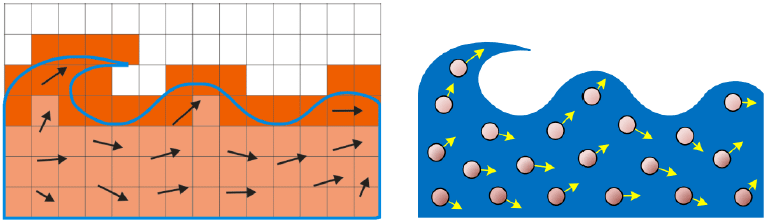
\includegraphics[scale=0.5]{images/gridBasedParticleBased}
        \caption{
            Grid based, Particle based simulation \cite{gridBasedParticleBased}
        }
        \label{fig:gridBasedParticleBased}
    \end{figure}


    \section{SPH metoda}\label{sec:sph-metoda}

    \subsection{Općenito o metodi}\label{subsec:opcenito-o-metodi}

    SPH\cite{SPHmethod} (Smoothed Particle Hydrodynamics) metoda je računska metoda koja se koristi za simulaciju fluida.
    Ova metoda je bazirana na česticama, pri čemu svaka čestica predstavlja mali volumen fluida.
    SPH metoda izračunava fizikalna svojstva fluida na temelju međučestičnih interakcija, omogućujući simulaciju fluida u složenim i nepravilnim prostorima bez potrebe za 2D poljem.

    \begin{itemize}
        \item \textbf{Osnovni princip:} U SPH metodi, prostor se ne dijeli na ćelije kao u metodama baziranim na mreži, već se koristi diskretna kolekcija čestica.
        Svaka čestica nosi informacije o fizikalnim svojstvima kao što su masa, brzina, gustoća i tlak.
        Interakcije između čestica izračunavaju se pomoću glatkih interpolacijskih funkcija, što omogućava kontinuirani prikaz fizikalnih veličina.
        \item \textbf{Prednosti:} Jedna od glavnih prednosti SPH metode je njena sposobnost da simulira fluide u složenim geometrijama i nepravilnim prostorima.
        Budući da ne koristi 2D polje, SPH metoda je fleksibilnija i može se lako prilagoditi različitim vrstama problema.
        Također, njena složenost u odnosu na broj čestica je manja nego kod metoda koje koriste 2D polje, posebno kada je gustoća čestica visoka.
        \item \textbf{Nedostaci:} Glavni nedostatak SPH metode je potreba za velikim brojem čestica kako bi se postigla visoka preciznost simulacije, što može povećati zahtjevnost simulacije i dodatno ju usporiti.
    \end{itemize}

    \newpage

    \subsection{Koraci simulacije}\label{subsec:koraci-simulacije}

    \paragraphnewline{Inicijalizacija simulacije}
    Na samom početku simulacije potrebno je definirati osnovne parametre koji će utjecati na ponašanje simulacije.
    Ovi parametri uključuju jačinu viskoznosti, koja određuje otpor tekućine prema promjeni oblika, te koeficijente međučestičnog odbijanja i privlačenja, koji utječu na način na koji se čestice međusobno odbijaju ili privlače.
    Osim toga, potrebno je definirati početne uvjete simulacije, kao što su početne pozicije i brzine čestica, kao i rubne uvjete koji definiraju granice simulacijskog prostora.
    Također, određuju se fizičke konstante kao što su gravitacija i koeficijenti pritiska, koji će biti korišteni u daljnjim koracima simulacije.

    \paragraphnewline{Traženje susjeda}
    Prvi ``pravi`` korak simulacije je traženje susjeda za svaku česticu.
    Susjedi su čestice koje se nalaze unutar određenog radijusa od ciljne čestice, i vrlo je važno znati njihove pozicije kako bi se na čestice mogle primijeniti sile koje ovise o udaljenosti, poput viskoznosti i pritiska.
    Najčešći pristup traženju susjeda je korištenje uniformne mreže ili 2D polja, gdje se svaka čestica na početku simulacije smješta u odgovarajuću ćeliju mreže.
    Kada se traže susjedi, provjeravaju se čestice u bliskim ćelijama mreže, što omogućava brzo i efikasno pretraživanje.
    Ova metoda značajno smanjuje broj potrebnih provjera udaljenosti između čestica, čime se optimizira cijeli proces simulacije.
    Uniformna mreža omogućava jednostavno indeksiranje i brzi pristup podacima, što je ključno za izvođenje simulacija u realnom vremenu.

    \begin{figure}[H]
        \centering
        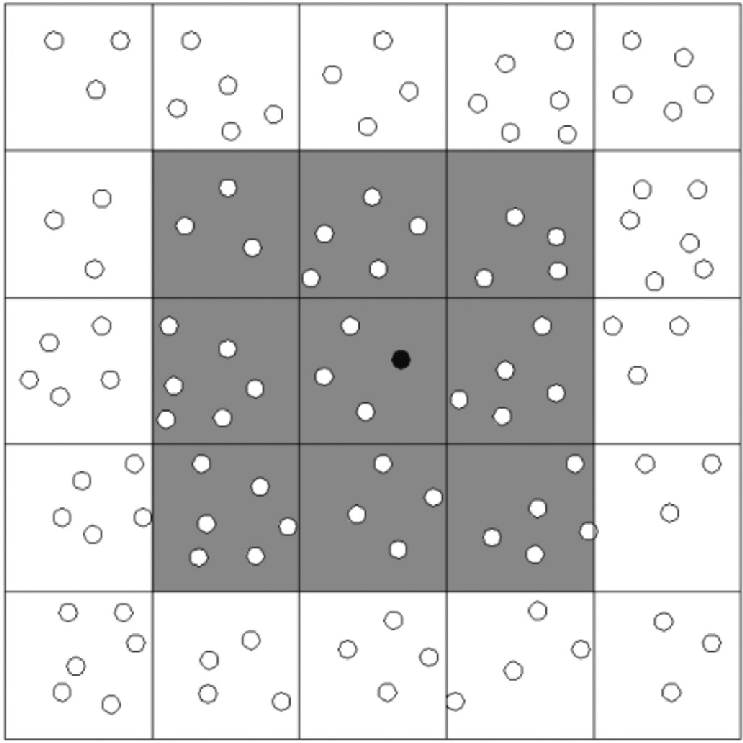
\includegraphics[scale=0.3]{images/Uniform-grid-searching-method}
        \caption{
            Uniform grid searching method \cite{uniformGridSearchingMethod}
        }
        \label{fig:uniformGridSearchingMethod}
    \end{figure}

    Drugi česti pristup traženju susjeda je korištenje stablastih struktura podataka, kao što su k-d stabla ili oktalna stabla.
    U ovom pristupu, čestice se organiziraju u hijerarhijsku strukturu stabla, gdje svaka čvor stabla predstavlja podskup čestica.
    Kada se traže susjedi za određenu česticu, pretraga se provodi spuštanjem niz stablo, čime se brzo identificiraju potencijalni susjedi.
    Ovaj pristup može biti vrlo učinkovit za velike skupove čestica jer smanjuje broj potrebnih provjera udaljenosti.

    \begin{figure}[H]
        \centering
        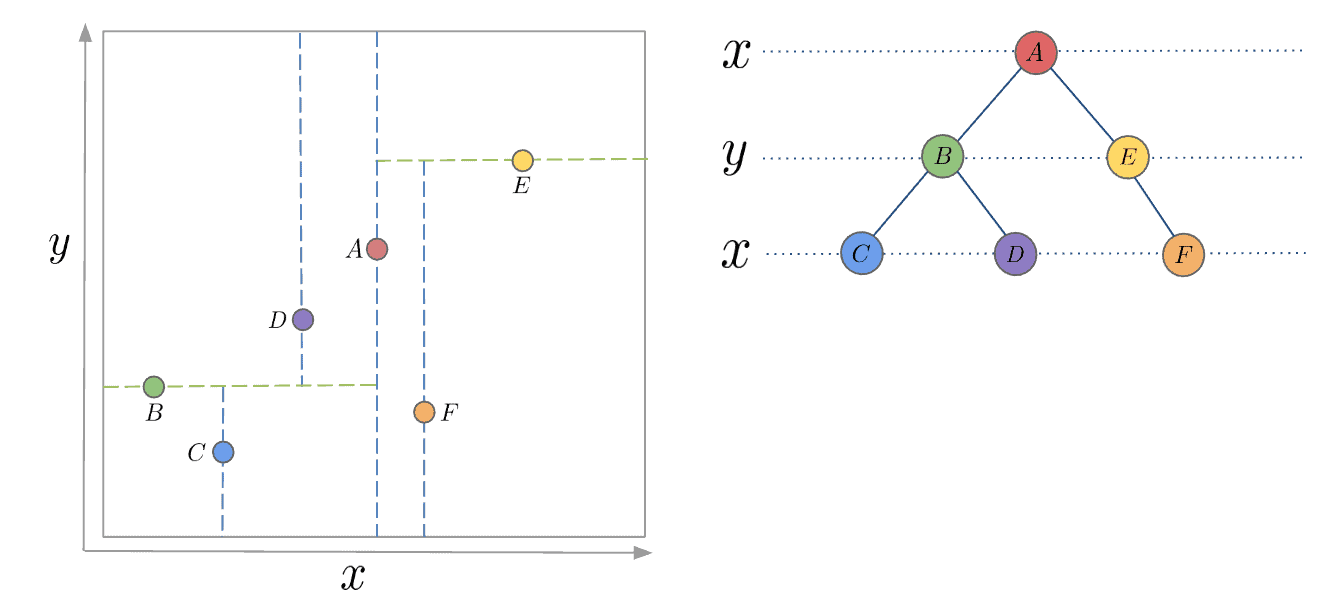
\includegraphics[scale=0.3]{images/kdtree}
        \caption{
            K-D stablo \cite{kdTree}
        }
        \label{fig:kdTree}
    \end{figure}

    Najjednostavniji, ali i najmanje efikasan pristup traženju susjeda je brute-force metoda, gdje se za svaku česticu provjerava udaljenost od svake druge čestice.
    Ovaj pristup ima kvadratnu složenost, što znači da se broj provjera eksponencijalno povećava s brojem čestica.
    Zbog toga je ovaj pristup previše spor za praktičnu upotrebu u simulacijama s velikim brojem čestica.


    \paragraphnewline{Računanje i primjena međučestičnih sila}

    Nakon pronalaska susjeda slijedi ključni korak u kojem se računaju međučestične sile.
    Ovo je najvažniji korak jer upravo ove sile su one koje pokreću čestice da se gibaju poput vode.
    Čestice ne smiju biti unutar jedne druge, ali se svejedno moraju kretati zajedno, a skupina čestica mora se ponašati kao kohezivna jedinica.
    Najbitnije sile u ovoj fazi su sile pritiska i sile viskoznosti.

    Prvo se računa gustoća, a zatim pomoću nje pritisak i onda nakon viskoza.

    Pritisak je bitan jer on tjera čestice jedne iz drugih kako nebi zapele jedna u drugu.
    \begin{figure}[H]
        \centering
        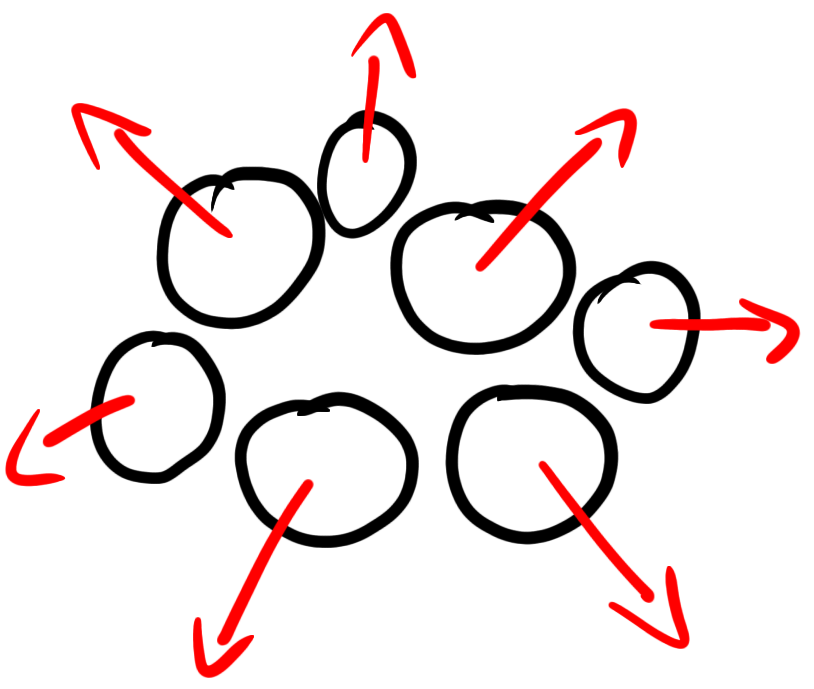
\includegraphics[scale=1]{images/pressureForce}
        \caption{
            Sile pritiska
        }
        \label{fig:pressureForce}
    \end{figure}

    \newpage
    S druge strane, viskoznost je sila koja drži čestice na okupu.
    Viskoznost povlači čestice jedne prema drugima, omogućujući im da se kreću kao jedinstvena masa.
    Što je viskoznost jača, fluid koji simuliramo bit će ``tvrđi`` i više će nalikovati krutini, jer će unutarnje sile biti toliko jake da će se vanjske sile poput gravitacije moći zanemariti.
    \begin{figure}[H]
        \centering
        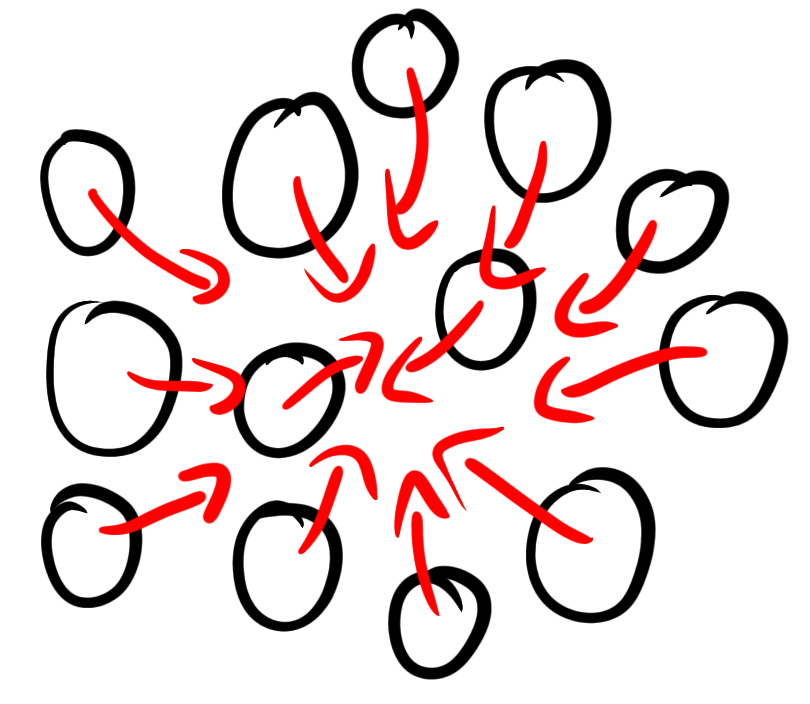
\includegraphics[scale=1]{images/viscoseForce}
        \caption{
            Sile viskoze
        }
        \label{fig:viscoseForce}
    \end{figure}

    Nakon što su sile pritiska i viskoznosti izračunate, primjenjuju se na svaku česticu kako bi se dobila nova brzina i položaj.
    Konačne pozicije i brzine čestica se ažuriraju na temelju ovih sila, omogućujući simulaciji da napreduje kroz vrijeme.

    Balansiranje ovih sila ključno je za postizanje realističnih simulacija fluida koje odgovaraju stvarnom ponašanju materijala.
    Kada su ove sile pravilno izračunate i primijenjene, simulacija će prikazivati prirodno gibanje tekućine, s česticama koje se pravilno međusobno odbijaju i privlače, oponašajući stvarno ponašanje vode ili drugih tekućina.

    \paragraphnewline{Upravljanje rubnim uvjetima i sudarima}
    Upravljanje rubnim uvjetima i sudarima predstavlja kritičan aspekt svake simulacije fluida, uključujući one koje koriste SPH metodu.
    Rubni uvjeti definiraju kako se fluid ponaša na granicama simulacijskog prostora, dok upravljanje sudarima osigurava realistične interakcije između fluida i čvrstih objekata ili granica.

    \begin{itemize}
        \item \textbf{Rubni uvjeti:} Postoji nekoliko vrsta rubnih uvjeta koji se mogu primijeniti u SPH simulacijama, uključujući:
        \begin{itemize}
            \item \textit{Dirichletovi rubni uvjeti:} Ovi uvjeti specificiraju vrijednosti funkcije (npr. brzine ili gustoće) na granicama simulacijskog prostora. Primjerice, u simulaciji fluida, brzina fluida na zidovima posude može biti postavljena na nulu kako bi se simuliralo stanje mirovanja.
            \item \textit{Neumannovi rubni uvjeti:} Ovi uvjeti specificiraju vrijednosti derivacija funkcije na granicama. U kontekstu simulacije fluida, ovo može značiti postavljanje gradijenta brzine ili tlaka na određene vrijednosti na granicama.
            \item \textit{Periodični rubni uvjeti:} Ovi uvjeti omogućuju česticama koje napuste jednu stranu simulacijskog prostora da se ponovno pojave na suprotnoj strani, stvarajući efekt beskonačnog prostora.
        \end{itemize}
        Pravilno postavljanje rubnih uvjeta ključno je za održavanje stabilnosti i realizma simulacije.
        Primjerice, u simulacijama gdje fluid dodiruje čvrste zidove, potrebno je osigurati da fluid ne procuri (``clippa``) kroz zidove i da se ponaša u skladu s očekivanim fizikalnim zakonima.

        \item \textbf{Upravljanje sudarima:} U simulacijama fluida, sudari mogu nastati između čestica fluida, kao i između čestica fluida i čvrstih objekata. Postoji nekoliko metoda za upravljanje sudarima:
        \begin{itemize}
            \item \textit{Phantom particles (fantomske čestice):} Ova metoda uključuje postavljanje dodatnih čestica duž granica čvrstih objekata. Fantomske čestice služe za simulaciju sile odbijanja, osiguravajući da čestice fluida ne prodiru kroz granice.
            \item \textit{Boundary handling (upravljanje granicama):} Ova metoda koristi posebne algoritme za detekciju i odgovor na sudare čestica fluida s granicama simulacijskog prostora. Na primjer, može se koristiti refleksija brzina kako bi se simulirao odbijanje fluida od zidova.
            \item \textit{Friction and adhesion (trenje i adhezija):} Ove sile igraju važnu ulogu u simulaciji interakcija između fluida i čvrstih površina. Trenje može smanjiti brzinu fluida pri kontaktu sa zidom, dok adhezija može uzrokovati da fluid ``prianja`` uz površine, što je važno za simulaciju efekata poput mokrih površina.
        \end{itemize}

        Upravljanje rubnim uvjetima i sudarima zahtijeva balansiranje između preciznosti i računalne efikasnosti.
        Pravilna implementacija ovih aspekata ključna je za stvaranje realističnih i stabilnih simulacija fluida koje se mogu koristiti u različitim aplikacijama, od računalne grafike do inženjerskih simulacija.


    \end{itemize}


    \chapter{Programska implementacija}\label{ch:programska-implementacija}

    U ovom poglavlju detaljno će biti opisani programske koraci implementacije SPH simulacije fluida koristeći Unity i C\#.
    Fokus će biti na osnovama Unity okruženja i Unity fizičkog simulatora, što će omogućiti razumijevanje integracije SPH metode u Unity okruženje.

    \section{Osnove Unity okruženja}\label{sec:osnove-unity-okruzenja}

    Unity je moćan razvojni alat koji omogućava stvaranje igara i simulacija u 2D, 2.5D i 3D okruženjima. Njegova fleksibilnost i pristupačnost čine ga idealnim izborom za razvoj složenih fizikalnih simulacija kao što je SPH metoda za simulaciju fluida.

    \subsection{Unity Editor}\label{subsec:unity-editor}
    Unity Editor je glavno razvojno okruženje koje omogućava korisnicima da dizajniraju, razvijaju i testiraju svoje aplikacije.
    Editor se sastoji od nekoliko ključnih komponenti:
    \begin{itemize}
        \item \textbf{Scene View:} Omogućava pregled i uređivanje scena igre.
        U ovom prikazu mogu se postavljati objekti, prilagođavati njihove pozicije, rotacije i veličine, te dodavati komponente.
        \item \textbf{Game View:} Omogućava pregled igre onako kako će je korisnik vidjeti kada je pokrene.
        Ovaj prikaz se koristi za testiranje i debugiranje.
        \item \textbf{Hierarchy Window:} Prikazuje sve objekte u sceni u hijerarhijskom prikazu.
        Ovdje se mogu organizirati objekti, stvarati roditeljsko-dječji odnose i upravljati strukturom scene.
        \item \textbf{Inspector Window:} Omogućava pregled i uređivanje svojstava odabranih objekata.
        Ovdje se mogu dodavati komponente te mijenjati vrijednosti postojećih komponenti i skripti.
        \item \textbf{Project Window:} Prikazuje sve resurse projekta, uključujući skripte, modele, teksture i zvukove.
        Ovdje se može upravljati resursima vašeg projekta.
    \end{itemize}

    \subsection{Komponente i GameObjecti}\label{subsec:komponente-i-gameobjecti}
    U Unityju, svaki objekt u sceni je GameObject.
    GameObjecti mogu imati različite komponente koje određuju njihovo ponašanje i izgled.
    Neke od ključnih komponenti uključuju:
    \begin{itemize}
        \item \textbf{Transform:} Svaki GameObject ima komponentu Transform koja pohranjuje informacije o poziciji, rotaciji i skali objekta.
        \item \textbf{Rigidbody:} Komponenta koja omogućava fizičku simulaciju objekta, uključujući gravitaciju, sile i sudare.
        \item \textbf{Collider:} Komponenta koja definira oblik objekta za detekciju sudara.
        Postoje različite vrste collidera, uključujući Box Collider, Sphere Collider i Mesh Collider, ovisno o objektu na koji stavljamo collider taj tip ćemo koristiti.
        \item \textbf{Script:} Komponente koje dodaju prilagođeno ponašanje objektima koristeći C\# skripte.
    \end{itemize}

    \subsection{Skripte u C\#}\label{subsec:skripte-u-c}
    Unity koristi C\# kao glavni programski jezik za razvoj skripti.
    Skripte omogućavaju programerima da definiraju prilagođeno ponašanje za GameObjecte.
    Neke ključne značajke skripti u Unityju uključuju:
    \begin{itemize}
        \item \textbf{Monobehaviour:} Svi skriptni objekti koji žele biti povezani s GameObjectima trebaju naslijediti klasu Monobehaviour.
        Ova klasa omogućava pristup osnovnim metodama životnog ciklusa kao što su Start, Update, FixedUpdate i LateUpdate, koje se zovu u određeno vrijeme ciklusa.
        \item \textbf{Metode životnog ciklusa:} \textit{Start} se poziva jednom kada se skripta prvi put pokrene, \textit{Update} se poziva jednom po taktu, \textit{FixedUpdate} se poziva na fiksnim vremenskim intervalima i koristi se za fiziku, dok se \textit{LateUpdate} poziva nakon svih Update metoda i koristi se za finaliziranje kretanja objekata.
        \item \textbf{Upravljanje komponentama:} Skripte mogu dodavati, uklanjati i mijenjati komponente GameObjecta, omogućavajući dinamičko ponašanje tijekom igre.
    \end{itemize}

    \section{Osnove Unity fizičkog simulatora}\label{sec:osnove-unity-fizickog-simulatora}

    Unity fizički simulator omogućava realističnu simulaciju fizikalnih interakcija među objektima.
    Ovaj simulator koristi komponente kao što su Rigidbody i Collider za upravljanje fizikalnim svojstvima objekata i detekciju sudara.

    \subsection{Rigidbody komponenta}\label{subsec:rigidbody-komponenta}
    Rigidbody komponenta dodaje fizikalna svojstva GameObjectu, omogućavajući mu da reagira na gravitaciju, sile i sudare.
    Ključne postavke Rigidbody komponente uključuju:
    \begin{itemize}
        \item \textbf{Mass:} Masa objekta koja utječe na to kako se objekt ponaša pod utjecajem sila.
        \item \textbf{Drag:} Otpornost na kretanje koja usporava objekt.
        \item \textbf{Angular Drag:} Otpornost na rotaciju.
        \item \textbf{Use Gravity:} Opcija koja određuje hoće li objekt biti pod utjecajem Unityjevog gravitacijskog simulatora.
        \item \textbf{Is Kinematic:} Ako je omogućeno, objekt neće biti pod utjecajem fizikalnih sila, već će se njime upravljati isključivo putem skripti.
    \end{itemize}

    \subsection{Collider komponenta}\label{subsec:collider-komponenta}
    Collider komponenta definira oblik objekta za detekciju sudara.
    Postoji nekoliko vrsta collidera koje ćemo koristiti ovisno o izgledu objekta ili slučaja korištenja u kojem se nalazimo:
    \begin{itemize}
        \item \textbf{Box Collider:} Pravokutni collider koji definira objekt kao kutiju, Kutija u nekoj igri.
        \item \textbf{Sphere Collider:} Kuglasti collider koji definira objekt kao sferu, Lopta u nogometnoj igri.
        \item \textbf{Capsule Collider:} Collider u obliku kapsule, Igrač u pucačkim igrama.
        \item \textbf{Mesh Collider:} Collider koji koristi mrežu (mesh) za definiranje složenih oblika.
    \end{itemize}

    Collideri omogućuju detekciju sudara i interakciju među objektima.
    Kada se dva collidera sudare, Unity fizički simulator izračunava reakcije temeljem fizikalnih svojstava objekata.

    \subsection{Simulacija fluida u Unityju}\label{subsec:simulacija-fluida-u-unityju}
    Za implementaciju SPH metode za simulaciju fluida u Unityju, potrebno je koristiti prilagođene skripte koje definiraju ponašanje čestica fluida.
    Ključni koraci uključuju:
    \begin{itemize}
        \item \textbf{Inicijalizacija čestica:} Postavljanje početnih pozicija, brzina i svojstava čestica.
        \item \textbf{Traženje susjeda:} Korištenje algoritama za brzo traženje susjeda unutar određenog radijusa.
        \item \textbf{Izračun međučestičnih sila:} Primjena pritiska, viskoznosti i drugih sila na temelju udaljenosti među česticama.
        \item \textbf{Ažuriranje položaja:} Korištenje numeričkih metoda za integraciju i ažuriranje položaja i brzina čestica kroz vrijeme.
        \item \textbf{Upravljanje sudarima:} Implementacija algoritama za detekciju i odgovor na sudare između čestica i s rubnim uvjetima.
    \end{itemize}

    Ove osnove Unity okruženja i fizičkog simulatora postavljaju temelje za razumijevanje kako implementirati kompleksne fizikalne simulacije poput SPH metode. Daljnji koraci uključuju detaljnu implementaciju svakog od ovih aspekata kako bi se postigla realistična simulacija fluida.

    \section{Čestica}\label{sec:cestica}


    \section{Gustoća}\label{sec:gustoca}


    \section{Pritisak}\label{sec:pritisak}


    \section{Viskoza}\label{sec:viskoza}


    \section{Rezultantna sila}\label{sec:rezultantna-sila}


    \bibliography{literatura}
    \begin{sazetak}
        sažetak na hrvatskom
    \end{sazetak}
    \begin{kljucnerijeci}
        ključne riječi na hrvatskom
    \end{kljucnerijeci}
    \begin{abstract}
        abstract in English
    \end{abstract}
    \begin{keywords}
        keywords in English
    \end{keywords}
\end{document}